\subsection{Molekulare Zustandssume (idealisierter Fall)}
\label{subsec:MolekulareZustandssume(idealisierterFall)}
\begin{sectionbox}\nospacing
  TD-Funktionen können durch Zustandsummen ausgedrückt werden, dies ist aber nur nützlich, falls die Zustandssummen berechenbar sind.\\
  \imp{Annahme} die grosse Anzahl der Systeme/Einheiten in einem Ensemble werden ähnliche/gleiche thermodynamische Eigenschaften
  aufweisen. Die Temperatur in einem Bad im Glg. wird an einer Stelle nicht plötzlich komplett verschieden sein vom Rest des Bades.\\
  $\Rightarrow$ die thermodynamischen Eigenschaften $\obs{A}$ der Einheiten des Ensembles sind representativ für die thermodynamischen
  Eigenschaften des Ensembles.\\
  $\Rightarrow$ versuche die Zustandsumme des Ensemble $\Zz$ mit der \rdb{molekularen Zustandssumme} $\zz$ der einzelnen Mitglieder des
  Ensembles, in Verbindung zu setzen.
\end{sectionbox}
\begin{defnbox}\nospacing
  \begin{defn}[Idealisiertes System]\label{defn:idealSys}\leavevmode\\
  Um die Zustandssumme $\Zz$ mit der molekularen Zustandssumme $\zz$ in verbindung zu setzen, die die einzelnen Mitglieder (Atome, Moleküle,
  Oszillatoren,\ldots) des Ensembles beschreibt, limitiert sich unsere Betrachtung auf idealisierte Systeme:
    \begin{circlelist}
      \item System besteht aus $\idxN$ nicht W.W. Teilchen $\Longleftrightarrow$ ideales Gas siehe \cref{subsec:Thermodynamische_Zustandsgleichungen}\label{circl:keineWW}
      \item Keine Koppelung der Bewegungsformen (z.B. Rotation, Vibration, \ldots) innerhalb eines Molekül/einer Einheit des Ensembles.
      \label{circl:TrennungDerBewegungsformen}
      \item Vernachlässigung weiterer Beiträge zur Energie (z.B. mag. Effekte der Kernspins auf die Energie des Moleküls)
      \item Alle Gasmoleküle des Ensembles sind gleich.\label{circl:ident}
    \end{circlelist}
  \end{defn}
\end{defnbox}
\begin{defnbox}\nospacing
  \begin{defn}[\\Zerlegung der Systemzustandssumem]
    \begin{flalign*}
      &\Zz=\prod_{\idxi}^{\idxN}\bdra{\zz_{\idxi}}{\normalfont{molekulare Zustandssumme}}\eqs{\circledItem{4}}\zz^{\idxN}\nalign
      &\EzrN\eqs{\circledItem{1}}\sum_{\idxi}^{\idxN}\Ez_{\idxi}^{\idxK(\idxr)}&\idxN\approx10^{24}\text{ Teilchen}
    \end{flalign*}
    \begin{flalign*}
    &\Ez_{\idxi}^{\idxK(\idxr)}:&\text{Energieeigenwert der stat. Schrödingergleichung}&\nalign
    &&\text{für das $\idxi$-te Molekül im $k$-ten Eigenzustand.}&&
    \end{flalign*}
  \end{defn}
\end{defnbox}
\begin{proofbox}
   \begin{proof}\imp{ by Example}
     \begin{align*}
       &\Zz\eqs{\text{kan. Zustd.summe}}\sum_{\idxn}\e^{-\betac(\Ez_{\mca}+\Ez_{\mcb})}\nalign
       &=\left(\e^{-\betac\Ez_{\mca_0}}+\e^{-\betac\Ez_{\mca_1}}+\cdots\right)\cdot\left(\e^{-\betac\Ez_{\mcb_0}}+\e^{-\betac\Ez_{\mcb_1}}+\cdots\right)\nalign
       &=(\zz_{\mca})(\zz_{\mcb})\eqs{\circledItem{4}}\zz^2
     \end{align*}
   \end{proof}
\end{proofbox}
\begin{sectionbox}[\rd{Un}unterscheidbare Moleküle]\nospacing
  Wenn sich die einzelnen Moleküle nicht eindeutig zuordnen lassen wie z.B. bei einem Kristall, in dem die Molekülpositionen fixiert sind, so
  müssen wir die molekulare Zustandssumme anpassen.
  \begin{align}
    \Zz=\frac{\zz^{\idxN}}{\idxN!}
  \end{align}
\end{sectionbox}
\begin{notebox}[Beispiel: harmon. Oszillatoren]
  \imp{Geg.}: 3 harm. Ozsillatoren $\mca$, $\mcb$ und $\mcc$ die die Eigenzustände 1,2,3 annehmen können.
  \begin{center}
    \begin{tabular}{ |c|c|c|c|c|c|c| } 
    \hline
    $\mca$ & 2 & 2 & 1 & 0 & 1 & 0 \\ 
    $\mcb$ & 1 & 0 & 2 & 2 & 0 & 1 \\ 
    $\mcc$ & 0 & 1 & 0 & 1 & 2 & 2 \\ 
    \hline
    \end{tabular}
  \end{center}
  Wenn die harm. Oszillatoren nicht unterscheidbar sind besteht allerdings kein Unterschscied zwischen den verscheidenen Anordnungen der
  Eigenwerte der Liste.
\end{notebox}
  \begin{defnbox}\nospacing
    \begin{defn}[Kanonische Molekülzustandssumme]
      \begin{align}
        \zz_{\idxi}=\sum_{\idxK}\e^{-\betac\Ez_{\idxi}^{\idxK}}\eqs{\circledItem{4}}\sum_{\idxK}\e^{-\betac\Ez^{\idxK}}
      \end{align}
    \end{defn}
  \end{defnbox}
\begin{sectionbox}[Berechnung der molekularen Zustandssumme]\nospacing
  Aus der Annahme der Trennung der Bewegungsformen \cref{circl:TrennungDerBewegungsformen} und
  \[\Ham(\text{"Gasmoleküle"})\cdot\Psi_{\idxK}=\Ez_{\idxK}\Psi_{\idxK}\]
  folgt das $\idxK$ eine zusammengesetzte Quantenzahl ist, die die Quantenzustände durchnumeriert und aus folgenden Beiträgen
  gebildet wird:
  \begin{circlelist}
      \item Abtrennung der Schwerpunktskoordinaten\\ $\rightarrow$ \tc{section}{Translation}.
      \item Abtrennung der Rotationsbewegung $\rightarrow$ \tc{section}{Rotation}.
      \item Lösung des internen Problems $\rightarrow$ \tc{section}{Vibration}.
      \item Elektronische Beiträge.
  \end{circlelist}
  \begin{align*}
    &\Rightarrow \idxK=\idxK(\nqz,\vqz,\Jqz,\Aqz)&\text{ mit }& \vqz=\left\{\vqz_{\idxi}\right\}
  \end{align*}
  \begin{align}
    \Aboxed{\Ez^{\idxK}&=\Eztrans+\Ezrot+\Ezvib+\Ezelek }\nalign
                         \Aboxed{\zz_{\text{m}}&=\zztrans\cdot\zz^{\text{intern}}=\zztrans\cdot\zzrot\cdot\zzvib\cdot\zzelek}
  \end{align}
\end{sectionbox}
\begin{sectionbox}[\subsubsection{Translation ($\corresponds$ Teilchen im 3D Kasten)}]\nospacing
  Kann durch die Energieeigenwerte eines Teilchens im 3D-Kasten beschrieben werden:
  \begin{align*}
    \Ez_{\nqz\in\Np}^{\text{1D-Box}}&=\frac{\nqz^2\hp^2}{8mL^2}=\frac{\nqz^2\hpr^2\pi^2}{2mL^2}\qquad\text{für 3D: }m=3, \nqz_x,\nqz_y,\nqz_z\nalign
                                      \Ez_{\nqz}^{\text{m-Box}}&=\sum_{\idxi}^{m}\Ez_{\idxi}=\Ez_{\text{GZst.}}\cdot\sum_{\idxi}^{m}\nqz_{\idxi}^2\nalign
                                                                 &=(\nqz_x^2+\nqz_y^2+\nqz_z^2)\frac{\hpr^2\pi^2}{2mL^2}
  \end{align*}
  \begin{align}
    \boxed{\zztrans=\sum_{\nqz}\e^{-\betac\Eztrans}}&&\nqz=\nqz_x,\nqz_y,\nqz_z
  \end{align}
\end{sectionbox}
\begin{sectionbox}[\subsubsection{Vibration ($\corresponds$ harm. Oszillator)}]\nospacing
  Kann durch die Energieeigenwerte des harmonischen Ozsillators beschrieben werden:
  \begin{align*}
    \Ez_{\vqz}=\hp\nu(\vqz+\frac{1}{2})=\hpr\omega(\vqz+\frac{1}{2})&&\omega=2\pi\nu=\sqrt{\frac{k}{m}}\nalign
    &&k:\text{ Federkonstante}
  \end{align*}
  \begin{align*}
    \zzvib&=\prod_{\idxi}^{\idxs}\left(\zz_{\vqz_{\idxi}}\right)\qquad
            \idxs=\begin{cases}
              3N-5 &\text{ für lin. Moleküle }\nalign
              3N-6 &\text{ für nichtlin. M.}
                  \end{cases}
  \end{align*}
  $\idxs$: Anzahl an Schwingungsfreiheitsgraden.
  \begin{align*}
  \zz_{\vqz_{\idxi}}^{\text{harm. Osz.}}&=\sum_{\vqz_{\idxi}=0}^{\infty}\e^{-\betac\Ez_{\vqz_{\idxi}}}=\sum_{\vqz_{\idxi}=0}^{\infty}\e^{-\betac\hpr\omega_{\idxi}(\vqz_{\idxi}+\frac{1}{2})}\nalign
    &=\e^{-\frac{\betac\hpr\omega_{\idxi}}{2}}\sum_{\vqz_{\idxi}=0}^{\infty}\e^{-\betac\hpr\omega_{\idxi}\vqz_{\idxi}}\nalign
    &\hspace{-3em}\eqs{\rd{\text{Geom. Reihe}}}\e^{-\frac{1}{2}\betac\hpr\omega_{\idxi}}\frac{1}{1-\e^{-\betac\hpr\omega_{\idxi}}}=\frac{\e^{-\frac{1}{2}\betac\hpr\omega_{\idxi}}}{1-\e^{-\betac\hpr\omega_{\idxi}}}
  \end{align*}
  \begin{align}
    \Aboxed{\zzvib&=\prod_{\idxi}^{\idxs}\left(\zz_{\vqz_{\idxi}}\right)=\prod_{\idxi}^{\idxs}\frac{\exp\{-\frac{1}{2}\betac\hpr\omega_{\idxi}\}}{1-\exp\{-\betac\hpr\omega_{\idxi}\}}}
  \end{align}
\end{sectionbox}
\begin{sectionbox}[\subsubsection{Rotation ($\corresponds$ starrer Rotator)}]\nospacing
    Kann durch die Energieeigenwerte eines starren Rotators
    beschrieben werden.\\
    \imp{Bemerkung}: wir betrachten hier der Einfachtheithalber nur den Spezialfall eines \imp{linearen} Moleküls.
    \begin{align*}
      &\boxed{\zzrot=\sum_{\Jqz}^{\infty}\left[\gfact_{\Jqz}\e^{-\betac\Ez_{\text{rot}}^{\Jqz}}\right]=\sum_{\Jqz}^{\infty}\left[(2\Jqz+1)\e^{-\betac\Ez_{\text{rot}}^{\Jqz}}\right]}\nalign
      &\Ez_{\text{rot}}^{\Jqz}=\Jqz(\Jqz+1)\frac{\hpr^2}{2I}\qquad I:\text{ Trägheitsmoment}
    \end{align*}
    \rdb{Entartungsfaktor} $\gfact_{\Jqz}=\underbrace{2\Jqz+1}_{\mathclap{\qz{M}_{\Jqz}=-\Jqz,\ldots,0,\ldots,+\Jqz}}$ der Energien $\Ez_{\text{rot}}^{\Jqz}$.
\end{sectionbox}
\begin{sectionbox}[\subsubsection{Elektronische Beiträge ($\corresponds$ Elektr. Schrdöd. Gl.)}]\nospacing
    Kann durch die Energieeigenwerte der elektonischen Schrödingergleichung beschrieben werden (sehr kompliziert).
    \begin{align}
      \zzelek=\sum_{\Aqz}\left[\gfact_{\Aqz}\e^{-\betac\Ez_{\text{el}}^{\Aqz}}\right]&&\gfact_{\Aqz}:\text{ Entartungsfaktor des}
    \end{align}
    Verschiebt man die Energieskala, sodass der Energienullpunkt beim Grundzustand liegt, so ergibt sich
    \begin{align*}
          \zzelek=\sum_{\Aqz}\left[\gfact_{\Aqz}\e^{-\betac(\Ez_{\text{el}}^{\Aqz}-\Ez_{\text{el}}^{\qz{0}})}\right]=\sum_{\Aqz}\left[\gfact_{\Aqz}\e^{\betac(\Ez_{\text{el}}^{\qz{0}}-\Ez_{\text{el}}^{\Aqz})}\right]
    \end{align*}
    Da meistens gilt $\Ez_{\text{el}}^{\qz{1}}\gg\Ez_{\text{el}}^{\qz{0}}$ wird häufig genähert:
    \begin{align}
      \zzelek=\sum_{\Aqz}\approx\gfact_{\qz{0}}\e^{-\betac\cdot0}=\gfact_{\qz{0}}\nalign
      \boxed{\zzelek=\gfact_{\qz{0}}=
      \begin{cases}
        1 & \text{für gewöhnliche Moleküle}\\
        2 & \text{für Radikale}\\
        3 & \text{für Ausnahmen z.B. Biradikale}
      \end{cases}}
    \end{align}
\end{sectionbox}
\begin{notebox}[Beispiel: zusammengesetzte kanonische Entropie]
\begin{wrapfigure}{l}{0.4\linewidth}	
  \begin{tikzpicture}[node distance=1cm,
      every node/.style={fill=notebox, font=\sffamily}]
    \node (TD)[rectangle, draw]          {Jede TD-Funktion};
    \node (Zzt)[rectangle, draw, below of=TD]          {$\Zz$};
    \node (Zz)[rectangle, draw, below of=Zzt]          {$\Zz=\frac{\zz^N}{N!}$};
    \node (zz)[rectangle, draw, below of=Zz]             {$\zz_{\text{m}}=\zztrans\cdot\zzrot\cdot\zzvib\cdot\zzelek$};
    % Draw edges
    \draw [ulc1,->] (TD) -- node {berechenbar durch} (Zzt);
    \draw [ulc2,->] (Zzt) -- node {Zerlegung} (Zz);
    \draw [ulc3,->] (Zz) -- node {Zerlegung} (zz);
  \end{tikzpicture}
\end{wrapfigure}
Mit Hife der Stirling Formel $\ln N!\approx N(\ln N-\ln\e)=N\ln N-N$ finden wir:
\begin{align*}
  &&\hspace{-3em}\Spot&\tc{ulc1}{=}\kb\ln\Zz+\kb\Tz \left(\pfrac{\ln\Zz}{\Tz}\right)\nalign
  &&&\hspace{-1em}\tc{ulc2}{\eqs{\tc{black}{\Zz=\frac{\zz}{N!}}}}\kb\cdot N\ln\zz\nalign
  &&&\hspace{-4em}-\kb\ln N!+\kb\Tz \left(\pfrac{\left(N\ln\zz-\ln N!\right)}{\Tz}\right)\nalign
  &&&\hspace{-3em}\Spot=\kb\ln\zz-\kb N\ln N+\kb\Tz N \pfrac{\ln\zz}{\Tz}
\end{align*}
\vspace{0.3cm}
\end{notebox}
\begin{figure}[H]\nospacing
  \centering{
  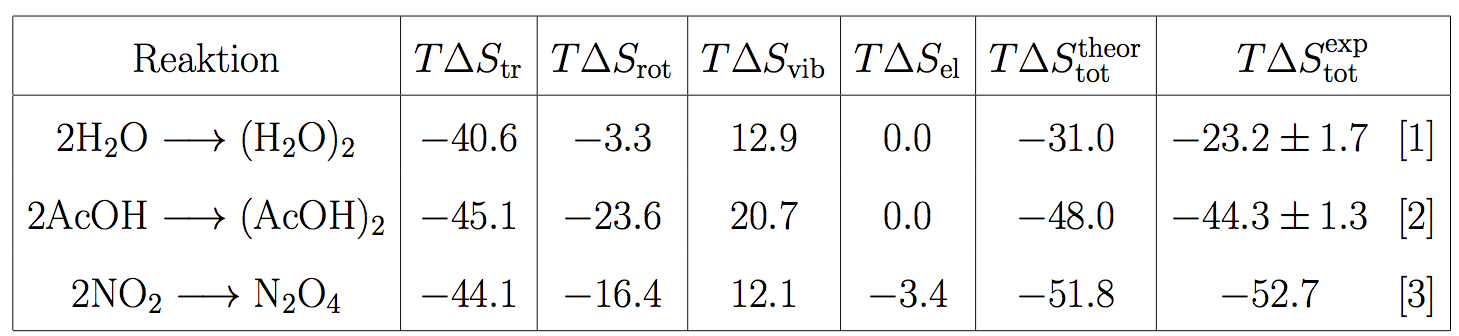
\includegraphics[width=\linewidth]{figures/zustandssummen/entropieBsp.png}
  }
\end{figure}
\vspace{-0.5cm}
\todo[inline]{Addd Kernspins (nicht in vorlesung vorgekommen) Für Proton, neutron I=1/2 (elektronen haben einen spin abner keinen Kernspin!)}
%%% Local Variables:
%%% mode: latex
%%% TeX-master: "../formularySPCS"
%%% End:
